\documentclass[11pt]{article}

% --------------------------------------------------
% Packages
% --------------------------------------------------
\usepackage[margin=1in]{geometry}
\usepackage{amsmath, amssymb, amsthm}
\usepackage{mathtools}
\usepackage{graphicx}
\usepackage{float}
\usepackage{enumitem}
\usepackage{hyperref}
\usepackage{xcolor}
\usepackage{tikz}
\usetikzlibrary{arrows.meta, shapes.geometric, positioning, calc}

% Pseudocode and algorithms
\usepackage{algorithm}
\usepackage{algpseudocode}

% Better fonts (optional)
\usepackage{lmodern}

% --------------------------------------------------
% Hyperref setup
% --------------------------------------------------
\hypersetup{
    colorlinks=true,
    linkcolor=blue,
    citecolor=blue,
    urlcolor=blue
}

% --------------------------------------------------
% Theorem-like environments
% --------------------------------------------------
\theoremstyle{definition}
\newtheorem{definition}{Definition}[section]
\newtheorem{theorem}{Theorem}[section]
\newtheorem{claim}{Claim}[section]
\newtheorem{remark}{Remark}[section]

\theoremstyle{proof}
% Proof environment is built-in via amsthm

% --------------------------------------------------
% Custom commands
% --------------------------------------------------
\newcommand{\Gen}{\mathsf{Gen}}
\newcommand{\Enc}{\mathsf{Enc}}
\newcommand{\Dec}{\mathsf{Dec}}
\newcommand{\negl}{\mathsf{negl}}

% --------------------------------------------------
% Document
% --------------------------------------------------
\begin{document}

\title{Public Key Crypto notes - 02}
\author{By contributors}
\date{February 16. 2026.}
\maketitle

% --------------------------------------------------
\section{Diffie-Hellman key exchange recap}
% --------------------------------------------------

\begin{itemize}
    \item Given: $p$ prime, $g \in \mathbb{Z}_p$ generator with large order $q = ord_p(g)$
    \item Randomly chosen $a, b \rightarrow g^a, g^b \rightarrow g^{ab}$ is the shared key
    \item Detailed description can be found in the previous lecture's notes.
    \item Typically, the generator $g$ is chosen so that $q = ord_p(g)$ is a large prime (i.e. $q \approx c \times p$, where $c = 2, 3, 5, \dots$ is typically a small constant)
\end{itemize}

\begin{remark}
	As $g^q \equiv 1 \pmod{p}$, the exponents $a, b$ can be computed on modulo $q$. Because of this, using $\mathbb{Z}_q$ is also a correct notation.
\end{remark}

\section{How to break this protocol?}

\begin{definition}[Discrete logarithm]
	Let $p$ be a prime and let $g \in \mathbb{Z}_p^*$ (the multiplicative group modulo $p$), typically with $g$ a generator of the group.
	For an element $y \in \mathbb{Z}_p^*$, the discrete logarithm of $y$ to the base $g$ modulo $p$ is the integer $x$ such that
	$$g^x \equiv y \pmod{p},$$
	where $0 \le x \le p-2$.
	We write this as
	$$x = \log_g y \pmod{p}.$$
	If $g$ is a generator of $\mathbb{Z}_p^*$, then such an $x$ exists and is unique modulo $p-1$.
\end{definition}

\begin{remark}
	In these notes, when we talk about $\log$, we are usually in base-2 logarithm ($\log_2$).
\end{remark}

\begin{claim}
	For a given $h = g^a$, computing $a = \log_q(h)$ is computationally hard.
\end{claim}

\subsection{Attacks against the Diffie-Hellman key exchange}

\subsubsection{Brute-force}

\begin{itemize}
	\item Running time: Size of the set of the possible expontents. $\mathcal{O}(q) = \mathcal{O}(p)$
	\item Given $p, q$ with order $q = ord_p(g)$ and $h = g^a$, try all $a' \in \mathbb{Z}_q^*$ values and check whether $g^{a'} = h$
	\item Space complexity: $\mathcal{O}(1)$
	\item This attack eventually succeeds, given enough time.
\end{itemize}

\subsubsection{Baby-step-giant-step algorithm}

Given $p, q$, where $q = ord_p(g)$, and $h = g^a$, let $a = i \times m + j$ with $m = \lceil\sqrt{q}\rceil, 0 \le i, j < m$. Then:

\begin{align}
	h &= g^a = g^{i \times m + j},\\
	g^j &= h \times (g^{-m})^i.	
\end{align}

\begin{figure}[h]
	\centering
	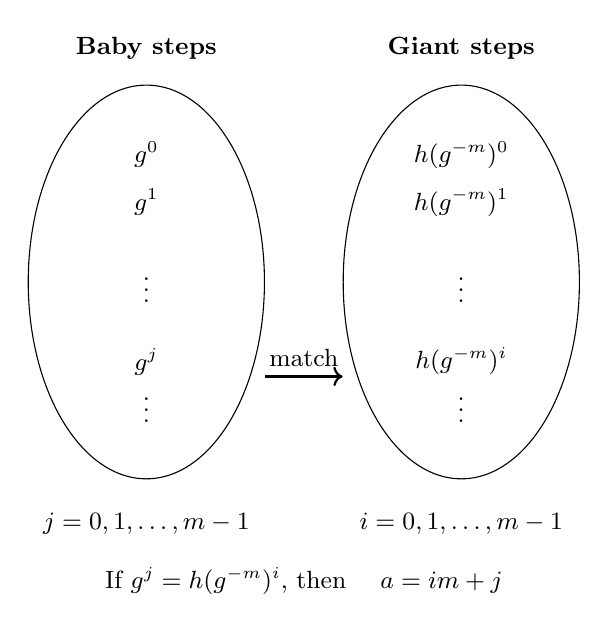
\begin{tikzpicture}[
		node distance=4cm,
		every node/.style={font=\small},
		set/.style={draw, ellipse, minimum width=3cm, minimum height=5cm},
		match/.style={->, thick}
		]
		
		% Left set: Baby steps
		\node[set] (baby) {};
		\node[above=0.2cm of baby] {\textbf{Baby steps}};
		\node at (baby.north) [below=0.6cm] {$g^0$};
		\node at (baby.north) [below=1.2cm] {$g^1$};
		\node at (baby.center) {$\vdots$};
		\node at (baby.south) [above=1.2cm] {$g^j$};
		\node at (baby.south) [above=0.6cm] {$\vdots$};
		
		\node[below=0.3cm of baby] {$j = 0,1,\dots,m-1$};
		
		% Right set: Giant steps
		\node[set, right of=baby] (giant) {};
		\node[above=0.2cm of giant] {\textbf{Giant steps}};
		\node at (giant.north) [below=0.6cm] {$h(g^{-m})^0$};
		\node at (giant.north) [below=1.2cm] {$h(g^{-m})^1$};
		\node at (giant.center) {$\vdots$};
		\node at (giant.south) [above=1.2cm] {$h(g^{-m})^i$};
		\node at (giant.south) [above=0.6cm] {$\vdots$};
		
		\node[below=0.3cm of giant] {$i = 0,1,\dots,m-1$};
		
		% Match arrow
		\draw[match] 
		([yshift=-1.2cm]baby.east) 
		-- node[above] {match}
		([yshift=-1.2cm]giant.west);
		
		% Conclusion
		\node[below=3.5cm of $(baby)!0.5!(giant)$] {
			If $g^j = h(g^{-m})^i$, then \quad $a = im + j$
		};
		
	\end{tikzpicture}
	\caption{Baby-step–giant-step algorithm: matching baby steps and giant steps to recover $a$.}
\end{figure}

\begin{itemize}
	\item Running time: $\mathcal{O}(m) = \mathcal{O}(\sqrt{q}) = \mathcal{O}(\sqrt{p})$
	\item Space complexity: Store both sets: $\mathcal{O}(m) = \mathcal{O}(\sqrt{q}) = \mathcal{O}(\sqrt{p})$
\end{itemize}

\begin{remark}
	There are other algorithms like Pollard's rho ($\rho$) algorithm with time complexity $\mathcal{O}(\sqrt{p})$ and with $\mathcal{O}(1)$ space complexity.
\end{remark}

Before presenting one last attack, we have to talk about key sizes (how large the prime $p$ should be).

\subsubsection{Key size}

Let's answer the question of how large should the prime $p$ be to achieve the same security level as AES-128, i.e. breaking would need $\approx 2^{128}$ time.

\begin{itemize}
	\item Brute-force: $\mathcal{O}(p) = \mathcal{O}(2^{\log_2 p}) \rightarrow \log p \approx 128$
	\item Baby-step-giant-step: $\mathcal{O}(\sqrt{p}) = \mathcal{O}(2^{\frac{1}{2}\log p}) \rightarrow \log p \approx 256$
\end{itemize}

With this clarification, we can move onto the next attack.

\subsubsection{Index calculus algorithm}

\begin{itemize}
	\item We won't give the precise details of the algorithm, only that it is the most efficient one for trying to find discrete logarithms.
	\item Running time: $\mathcal{O}(e ^{ (\sqrt[3]{\frac{64}{9}} + \epsilon) (\log p)^\frac{1}{3} (\log \log p)^\frac{2}{3}})$
	\item $\mathcal{O}(e ^{ (\sqrt[3]{\frac{64}{9}} + \epsilon) (\log p)^\frac{1}{3} (\log \log p)^\frac{2}{3}}) \rightarrow 2^{128} \rightarrow \log p \approx 3072$ 
\end{itemize}

\begin{remark}
	This is called a \emph{subexponential} running time.
	\begin{itemize}
		\item Exponential time: $\mathcal{O}(2^n)$
		\item Polynomial time: $\mathcal{O}(n^c)$
		\item $\mathcal{O}(n^c) < \mathcal{O}(e^{c \cdot n^{\frac{1}{3}}}) < \mathcal{O}(2^n)$
	\end{itemize}
\end{remark}

\begin{definition}[Hardness of the discrete logarithm problem]
	We say that the discrete logarithm problem is computationally hard if for all probabilistic polynomial time (PPT) adversary $A$, input size $n$ (i.e. $n = \log p$) and negligible function $negl(n)$:
	
	$$
	Pr[A(g^a) = a] \le negl(n)
	$$
\end{definition}

\begin{definition}[Computational Diffie-Hellman Problem]
	Given
	
	$$
	(g, g^a, g^b),
	$$
	
	for a randomly chosen generator $g$ and random
	
	$$
	a, b \in \{0, \ldots, q-1\},
	$$
	
	
	it is computationally intractable to compute the value
	
	$$
	g^{ab}.
	$$
\end{definition}

\begin{definition}[Hardness of the Computational Diffie--Hellman Problem]		
	We say that the Computational Diffie--Hellman problem (CDH) is hard if, for all security parameters $n$ (i.e., $n = \log q$) and for all PPT adversaries $A$,
	$$
	\Pr\big[ A(g, g^a, g^b) = g^{ab} \big] \le \mathrm{negl}(n),
	$$
	where $g$ is a generator of a cyclic group $G$ of order $q$, and $a, b \in_R \{0, \ldots, q-1\}$.
\end{definition}

\begin{definition}[Hardness of the Decisional Diffie--Hellman Problem]
	We say that the Decisional Diffie--Hellman problem (DDH) is hard if there exists no PPT adversary that can distinguish $g^{ab}$ from a random group element.
	
	Formally, DDH is hard if, for all security parameters $n$ and all PPT adversaries $A$,
	$$
	\left|
	\Pr\big[ A(g, g^a, g^b, g^{ab}) = 1 \big]
	-
	\Pr\big[ A(g, g^a, g^b, g^c) = 1 \big]
	\right|
	\le \mathrm{negl}(n),
	$$
	where $a, b, c \in_R \{0, \ldots, q-1\}$.	
\end{definition}

\subsubsection{Additional remarks}

Suppose that an adversary $A$ is given $p, q, g$. For given $r, s, z$, it outputs

$$
A(r, s, z) =
\begin{cases}
	1 & \text{if } z = g^{\log r \cdot \log s}, \\
	0 & \text{otherwise}.
\end{cases}
$$

\begin{remark}
	If the discrete logarithm problem is hard, that also means that the CDH problem is hard and vice-versa. There are also cases where the CDH problem is supposed to be hard, but the DDH problem is easy.
\end{remark}

\begin{remark}
	One can define the security of key exchange protocols and show that if the DDH problem is hard, then the Diffie-Hellman key exchange protocol is secure. We will make this fact clearer when we are discussing encryption protocols
\end{remark}

\section{Introduction to public key encryption schemes}

\begin{definition}[Public key encryption scheme]
	\item A Public Key Encryption (PKE) scheme is a triple $\Pi = (Gen, Enc, Dec)$, where:
	\begin{enumerate}
		\item $Gen$: Input: security parameter $1^n$ (in other words, an $n$ length string of $1$s), output: $(pk, sk)$ (public key, secret key)
		\item $Enc$: Input: $pk, m$, output: $c \leftarrow Enc_{pk}(m)$, where $\leftarrow$ denotes that $Enc$ is not necessarily deterministic
		\item $Dec$: Input: $sk, c$, output: $m$ or $\bot$, where $\bot$ is an error indicating an invalid ciphertext
	\end{enumerate}
\end{definition}

We require that --- except for a negligible probability --- if $(pk, sk) \leftarrow Gen(1^n)$ and $c \leftarrow Enc_{pk}(m)$, then $Dec_{sk}(c) = m$.

\end{document}
